\documentclass[a4paper, 10pt]{report}
\usepackage[italian]{babel}
\usepackage[T1]{fontenc}
\usepackage[utf8]{inputenc}
\usepackage{charter}
\usepackage{amsmath}
\usepackage{amsthm}
\usepackage{amsfonts}
\usepackage{graphicx}
\usepackage{wrapfig}
\usepackage{tcolorbox}
\usepackage{mathtools}
\usepackage{fancyhdr}

\usepackage{geometry}
\geometry{a4paper, left=2cm,right=2cm,top=2cm,bottom=2cm}

\pagestyle{fancy}
\lhead{}
\chead{}
\lhead{\bfseries Fondamenti dell'informatica}
\rhead{\bfseries 21 ottobre 2019}

\begin{document}

\subsection*{Proprietà di chiusura dei linguaggi regolari}

\paragraph*{Teorema} Se $\mathfrak{L}$ è un linguaggio regolare, allora anche la sua chiusura $\mathfrak{\overline{L}} = \Sigma^* \textbackslash \mathfrak{L}$ è regolare.

\begin{tcolorbox}
\paragraph*{Dimostrazione} Basta costruire un automa a stati finiti $\overline{M}=<Q, \Sigma, \delta, Q\textbackslash F, q_0>$ che legge $\mathfrak{L}$ -> gli stati finali sono opposti a quelli di $M$.
\end{tcolorbox}

\paragraph*{Corollario} $\mathfrak{L}_1 + \mathfrak{L}_2$ e $\mathfrak{L}_1 \cap \mathfrak{L}_2 = \overline{\overline{\mathfrak{L}_1} \cup \overline{\mathfrak{L}_2}}$ sono regolari.

\subsubsection*{Partizione di un insieme}
Una partizione $S$ è, dato un insieme $X$, una divisione di $X$ in sottoinsiemi, dette classi della partizione, che "coprono" X senza sovrapporsi. \\

\noindent \textbf{Definizione formale}: Una partizione $S = S_1 \cup ... \cup S_n$ è una collezione di sottoinsiemi tali che:
\begin{itemize}
\item[-] I sottoinsiemi non sono vuoti;
\item[-] L'unione di tutti i sottoinsiemi è l'insieme di partenza;
\item[-] Dati due sottoinsiemi (distinti) qualsiasi, questi sono disgiunti.
\end{itemize}

\noindent Una \textbf{classe di equivalenza} è una qualsiasi classe di $S$. Se $a \in S_i$, allora si può indicare la classe di equivalenza $S_i$ con $[a]_R$. Se il numero di classi è finito, si dice che $R$ è di indice finito.

\noindent Date due equazioni di equvalenza $R_1$ ed $R_20$, $R_1$ raffina $R_2$ se $\forall a [a]_{R_1} \subseteq [a]_{R_2}$.

\paragraph*{Teorema} Valgono le seguenti proprietà:
\begin{enumerate}
\item Dati un linguaggio $\mathfrak{L} \subseteq \Sigma^*$ e la funzione $R_\mathfrak{L} \subseteq \Sigma^* x \Sigma^*$, vale che $x R_\mathfrak{L} y$ se e solo se $(\forall z \in \Sigma^*)$ $(xz \in \mathfrak{L} \longleftrightarrow yz \in \mathfrak{L})$; 
\item Dati $M = <Q, \Sigma, \delta, q_0, F>$ e la funzione $R_M \subseteq \Sigma^* x \Sigma^*$, vale che $x R_M y$ se e solo se $\hat{\delta}(q_0, x)$ <-> $\hat{\delta}(q_0, y)$.
\end{enumerate}

\noindent Entrambe le proprietà sono quindi invarianti destre, in quanto $x R y \rightarrow \forall z xz R yz$.\\

\begin{tcolorbox}[title=\textbf{Invarianza destra}]
\paragraph*{Dimostrazione per proprietà 1} Siano $x, y \in \Sigma^*$ con $x R_L y$ se e solo se $(\forall z)$ $(xz \in \mathfrak{L} \longleftrightarrow yz \in \mathfrak{L})$ e sia $z \in \Sigma^*$. Dobbiamo dimostrare che $xz R_L yz$. 

La dimostrazione si fa per assurdo: Supponiamo che esiste $w$ tale che $xzw \in \mathfrak{L}$ e $yzw \notin \mathfrak{L}$. Ma se poniamo $zw = z$ allora abbiamo $xz \in \mathfrak{L}$ e $yz \notin \mathfrak{L}$. Questo però è l'opposto di quanto supposto sopra, quindi si ha un assurdo.
\\
\paragraph*{Dimostrazione per proprietà 2} Per questa dimostrazione basta fare delle prove sul seguente automa:

\begin{center}
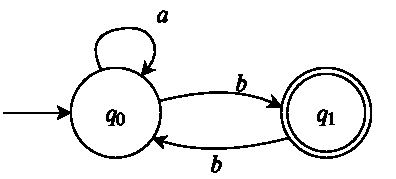
\includegraphics[scale=0.8]{1.pdf}
\end{center}
\end{tcolorbox}

\noindent Il seguente teorema è un risultato molto importante, infatti afferma che esiste un unico automa minimo in grado di riconoscere un linguaggio, e ci da anche una procedura per costruirlo. Questa esistenza di minimizzazione non sarà possibile per le grammatiche CF e per le macchine di Turing. 

\paragraph*{Teorema Myhill - Nerode}
	Le seguenti affermazioni sono equivalenti:
	\begin{enumerate}
		\item $L \in \Sigma^*$ è regolare;
		\item $L$ è l'unione di classi di equivalenza su $\Sigma^*$ indotte da una relazione invariante destra di indice finito;
		\item $R_L$ è di indice finito;
	\end{enumerate}

\begin{tcolorbox}
\paragraph*{Dimostrazione $(1) \rightarrow (2)$} L'obiettivo è dimostrare che $R_M$ è la relazione che soddisfa $(2)$.

Se $\mathfrak{L}$ è regolare esiste un automa a stati finiti tale che $\mathfrak{L}=\mathfrak{L}(M)$. Abbiamo quindi $\mathfrak{L}=\bigcup_{q\in F} \{x\in\Sigma^*:\hat\delta(q_0,x)=q\}$.
	
	Per definizione $xR_My \longleftrightarrow\hat\delta(q_0,x)=\hat\delta(q_0,y)$ è invariante destra e di indice finito in quanto $Q$ è finito. Quindi gli insiemi $\mathfrak{L}_q =\{x\in\Sigma^*:\hat\delta(q_0,x)=q\}$ costituiscono le classi di equivalenza della partizione indotta da $R_M$ e  il linguaggio $\mathfrak{L}=\bigcup_{q\in F}\mathfrak{L}_q$ è l'unione di queste classi di equivalenza. 
	
	Pertanto $\mathfrak{L}=\bigcup_{q\in F}\mathfrak{L}_q$ è un unione di classi di equivalenza indotte da una relazione invariante destra di ordine finito come volevamo dimostrare. \\
	
\paragraph*{Dimostrazione $(2)\Rightarrow(3)$} L'obiettivo è dimostrare che $R$ raffina $R_\mathfrak{L}$, ossia che $(\forall x\in\Sigma^*) ([x]_R\subseteq[x]_{R_\mathfrak{L}})$.

Dato che $R$ è una relazione di indice finito per (2), allora lo sarà anche $R_L$.\\
	
\paragraph*{Dimostrazione $(3)\Rightarrow(1)$} Costruiamo un $M'=\langle Q',\Sigma,\delta',q_0',F'\rangle$ dove:
	\begin{itemize}
		\item $Q' = \{[x]_{R_L}:x\in\Sigma^*\}$
		\item $q_0 = [\varepsilon]_{R_L}$
		\item $\delta'([x]_{R_L}, a) = [xa]_{R_L}, a\in\Sigma^*$
		\item $F'=\{[x]_{R_L}:x\in L\}$ 
	\end{itemize}

	Si dimostra per induzione su $|y|\geq0$ che $\hat\delta'([x]_{R_L},y)=[xy]_{R_L}$. Quindi
	\[
		\hat\delta'(q_0',x)=\hat\delta'([\varepsilon]_{R_L},x)=[\varepsilon x]_{R_L}=[x]_{R_L}
	\] 
	e pertanto 
	\[
		x\in L(M')\iff\hat\delta'(q_0',x)\in F'\iff [x]_{R_L}\in F' \iff x \in L
	\]
\end{tcolorbox}

\end{document}